
\section{Peer connectivity}

The question ``what are you taking this semester?'' may possibly be the most common phrase uttered in campus smalltalk within the first few weeks of a semester. But students' social lives do not solely exist in-person---social media dominates college social lives etc, v impt to consider [CITE]. The ``what are you taking'' question typically translates to social media in the form of the schedule image exported from Better CDCS posted to Facebook (e.g. Figure \ref{fig:cdcs-social}). There are several limitations to this model.

\begin{figure}[H]
  \centering
  \vspace{5pt}
  \begin{tabular}{c c}

    \begin{subfigure}[w]{7cm}
      \centering
      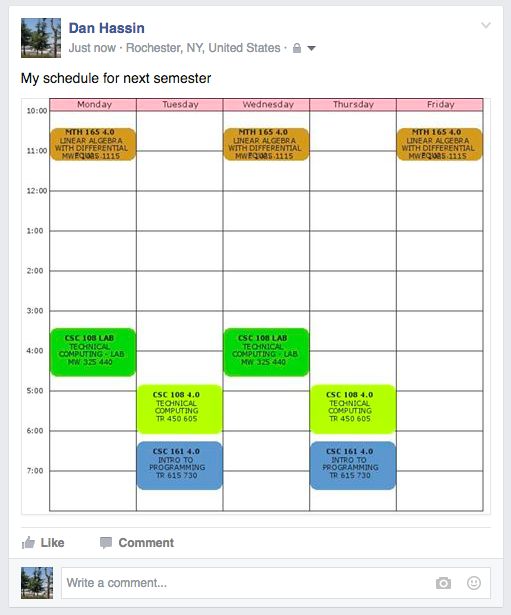
\includegraphics[width=6cm]{images/cdcs/social}
      \caption{Sharing a static schedule image generated by Better CDCS on Facebook} \label{fig:cdcs-social}
    \end{subfigure}

    \hspace{10pt}

    \begin{subfigure}[w]{7cm}
      \centering
      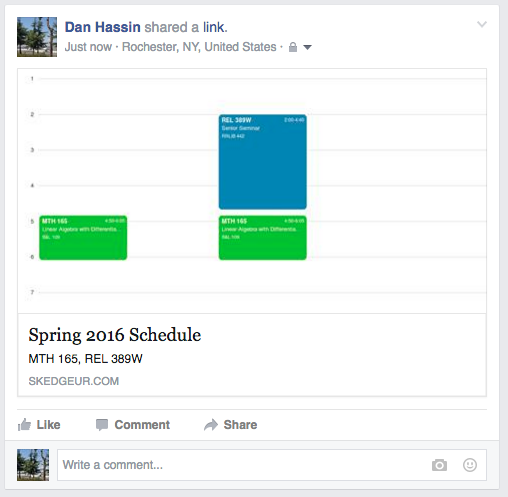
\includegraphics[width=6.1cm]{images/skedge/facebook}
      \caption{Sharing a Skedge schedule on Facebook, linked to the live and dynamic schedule share page on Skedge} \label{fig:sk-fb}
    \end{subfigure}

  \end{tabular}
  \caption{Comparison of sharing schedules on Facebook}
\end{figure}

\subsection{Limitations of the Facebook model, remedied by Skedge}

  \subsubsection{Static image vs. live site}

    As mentioned above, the schedules generated with Better CDCS cannot be shared publicly, and therefore students can only post a static image of their schedule at the time of posting. This excludes the possibility of edits to the schedule being reflected in the same post to their friends. Moreover, referencing courses (i.e. looking up more information on a course a friend is taking) is not very usable under this model as it requires a manual search.

    Skedge allows users to generate a public link (of the format \url{http://skedgeur.com/1234}, with the last four digits being a random ID for that schedule) to a view-only, larger version of their schedules (see Figure \ref{fig:sk-share}). If a user visiting others' share pages also has their schedule saved on Skedge, the option to ``overlay'' the user's schedule ontop of the share page's schedule is available, making it easier for friends to find common free time (see Figure \ref{fig:sk-overlay}).

    When this link is posted on Facebook, Skedge will include a rendered image of the schedule in the post, maintaining the element of visual bait with posting a static image (see Figure \ref{fig:sk-fb}).

    \begin{figure}[H]
      \centering
      \begin{tabular}{c c}
        \vspace{10pt}

        \begin{subfigure}[w]{10cm}
          \centering
          \fbox{
            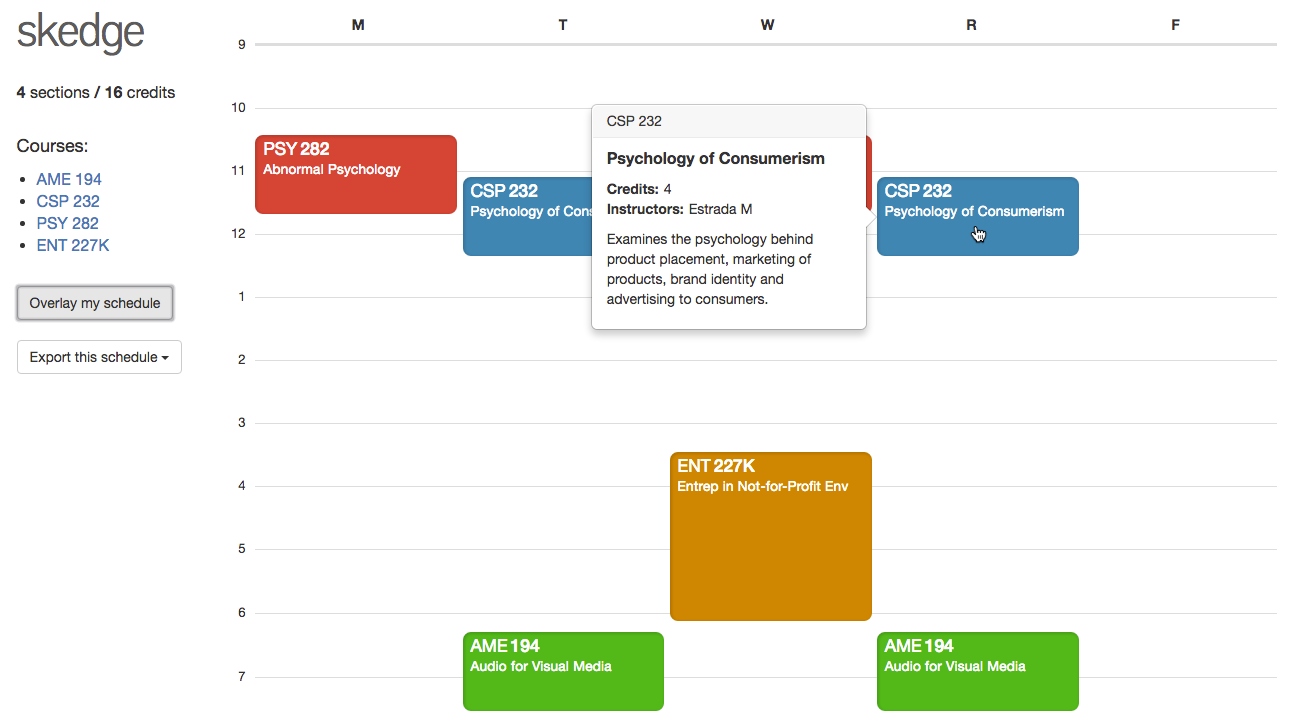
\includegraphics[width=1.00\textwidth]{images/skedge/share}
          }
          \caption{Skedge's schedule ``share'' page. Hovering over a course shows information about it, and clicking searches for it.} \label{fig:sk-share}
        \end{subfigure} \vspace{10pt}\\
        
        \begin{subfigure}[w]{10cm}
          \centering
          \fbox{
            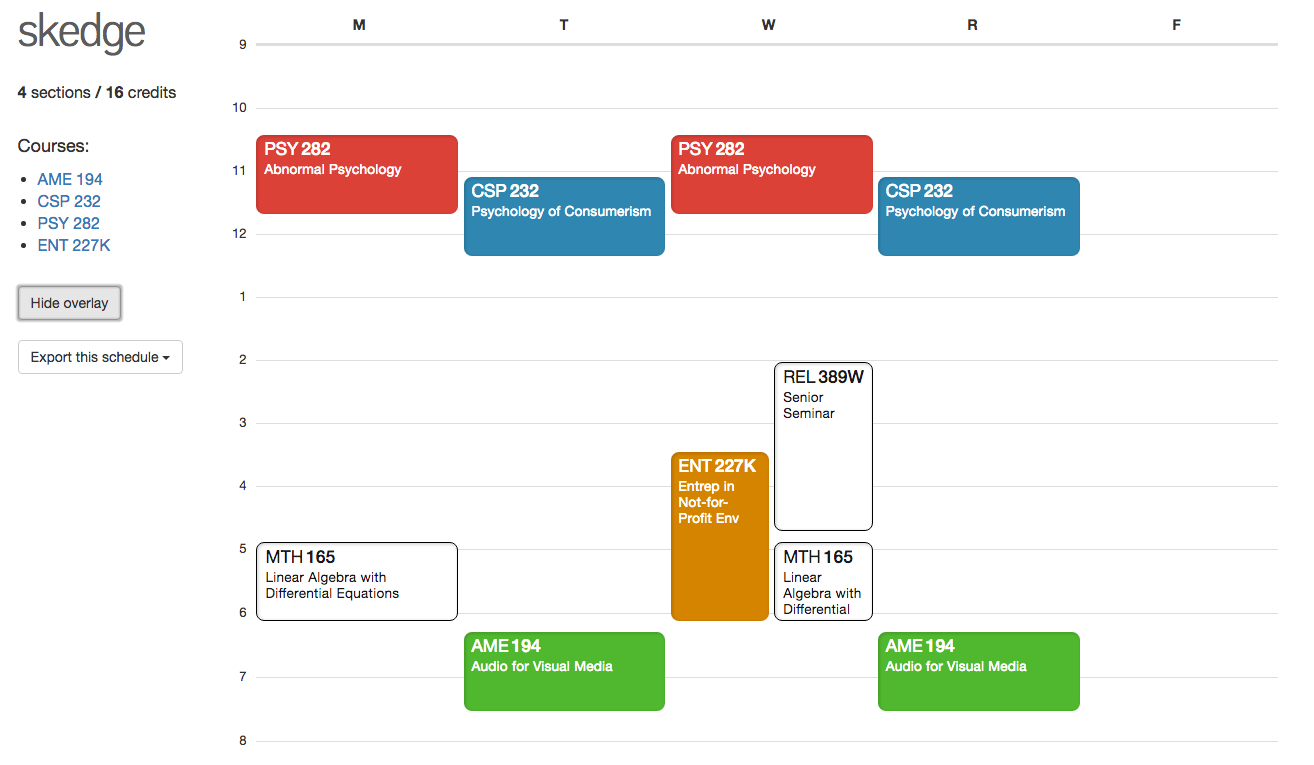
\includegraphics[width=1.00\textwidth]{images/skedge/share-compare}
          }
          \caption{The ``overlay'' feature enabled, superimposing the user's schedule over the share page's schedule.} \label{fig:sk-overlay}
        \end{subfigure}
      \end{tabular}
      \caption{Skedge's per-schedule share page}
    \end{figure}


  \subsubsection{Robustness of finding courses taken by peers}

  The Facebook model stimies users from finding courses peers are taking in several ways. It

  \begin{enumerate}
    \item requires that \textbf{a)} peers share their schedules on Facebook publicly and \textbf{b)} the user incidentally checks Facebook while that post is still deemed relevant via Facebook's algorithms.

    \item is unorganized, as schedules are spread across space and time (different posts and profiles).

    \item is only effective for the \emph{current semester}. It can be very difficult for students seeking advice (or even academic help) for a specific class to find others who had taken it before.

    \item is \emph{schedule}-oriented, not \emph{search}-oriented. Course discovery can only happen from seeing peers' schedules, not from browsing and finding classes that their peers may be taking.

  \end{enumerate}

  \noindent Solving these issues requires platform infrastructure external to Facebook, but Facebook's ubiquity is invaluable. Since Skedge already saves and archives users' schedules and Facebook has an integration API, building this platform into Skedge was the natural solution.

%figure
 
\subsection{Skedge Social}

The \emph{Skedge Social} platform aims to leverage existing social media paradigms (e.g. \emph{news feed}, \emph{likes}, and \emph{requests}) to more seamlessly give users answers to the questions alluded to earlier---``what are my friends taking?'' and ``what do my friends recommend?''. Skedge Social currently only supports Facebook, which can be integrated with a single click (see Figure \ref{fig:sk-social-login}).
  
  \begin{figure}[H]
      \centering
      \fbox{
        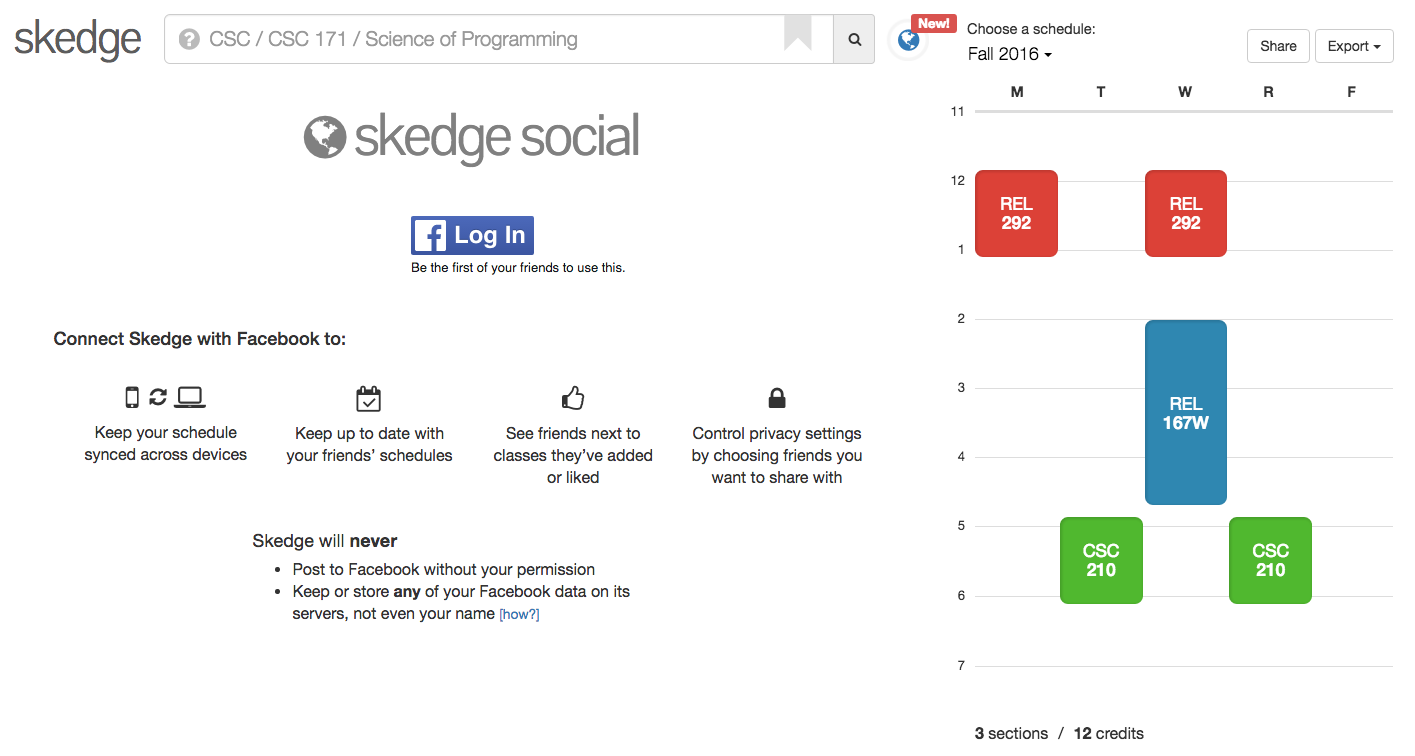
\includegraphics[width=9cm]{images/skedge/social-login}
      }
      \caption{Skedge Social landing page (\url{http://skedgeur.com/social}) for a user whose account has not yet been integrated with Facebook. Skedge Social appears in the context of the ordinary Skedge interface, and is accessible with the globe icon to the right of the searchbar.} \label{fig:sk-social-login}
    \end{figure}

  \subsubsection{Schedule feed}

  Immediately after logging in, the user will see the ``schedule feed,'' the list of the user's peers' current schedules (see Figure \ref{fig:sk-feed}). This takes from a familiar paradigm of the \emph{feed} in social networks, which is routinely scrolled for updates.[1] For each schedule, the user can visualize their own schedule side-by-side (using with the same ``overlay'' mechanic explained earlier), access the Facebook profile of the schedule's owner, and see the list of courses that user likes.

  This has the advantage of organizing and persisting peers' schedules, solving the first three issues of the ``Facebook post'' model listed above.
      
    \begin{figure}
      \centering
      \fbox{
        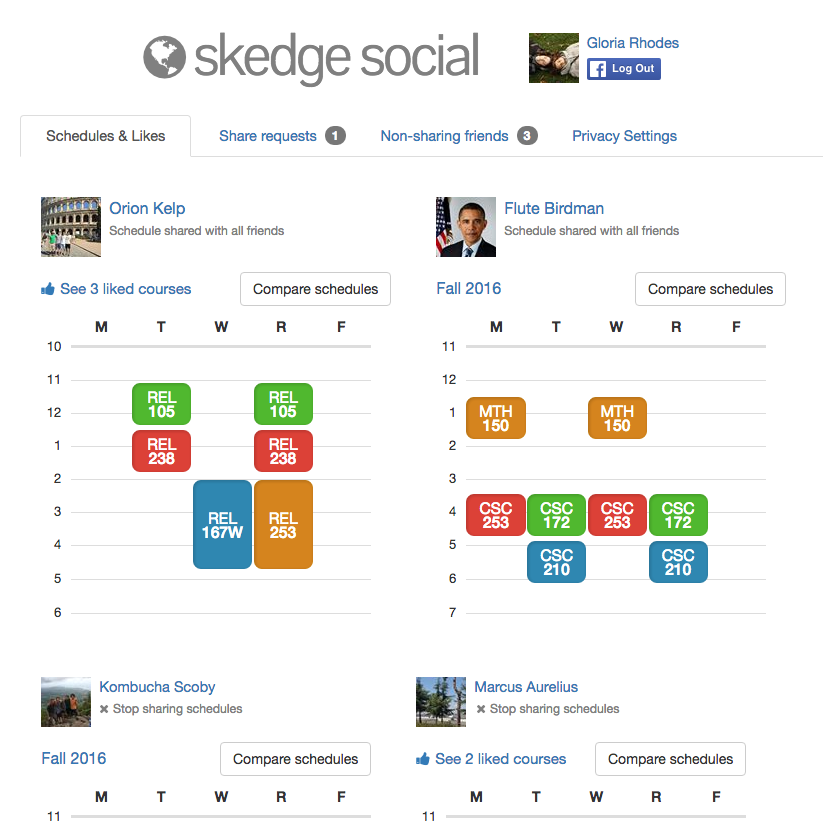
\includegraphics[width=9cm]{images/skedge/social}
      }
      \caption{Skedge Social's schedule feed (the default of four tabs) for a user who has integrated their Skedge account with Facebook. The user can toggle between a peer's schedule and the list of their \emph{liked} courses.} \label{fig:sk-feed}
    \end{figure}
  
  \subsubsection{Search result integration}

  Skedge Social also integrates into course search results, showing the user any other peers on the platform who are taking, have taken, or \emph{liked} courses in the results list (see Figure \ref{fig:sk-social-course}). This has several advantages, which solve the last ``Facebook post'' model issue listed above:

  \begin{itemize}

  \item It enhances the user's social engagement and allows them to better keep up with peers.
  \item It promotes and facilitates communication for users either seeking or soliciting advice regarding courses (sending a Facebook message is merely two clicks away).
  \item It brings attention to courses which are particularly popular or liked among the user's community of peers, increasing the chances of serendipitous course discovery.

  \end{itemize}

    \begin{figure}
      \centering
      \fbox{
        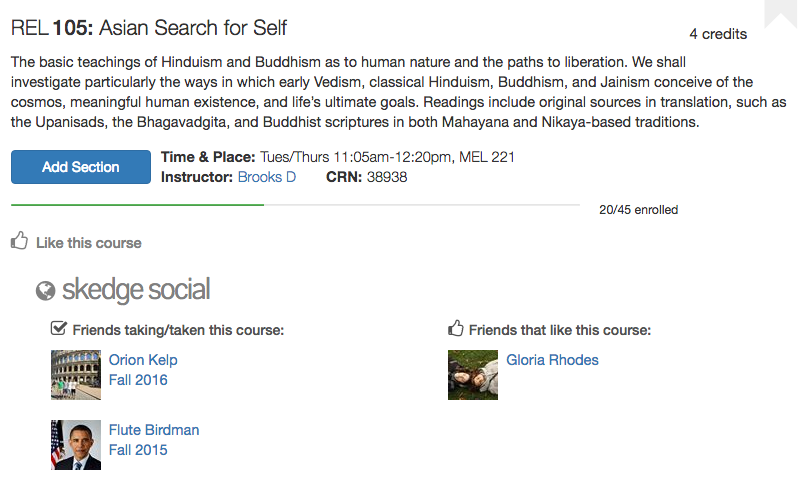
\includegraphics[width=12cm]{images/skedge/social-course}
      }
      \caption{Skedge Social integrating into a course search result} \label{fig:sk-social-course}
    \end{figure}

  \subsubsection{Personal schedule synchronization}

  In Section 2.1.4, discussing the disadvantages of Better CDCS's decentralized schedule store, I mentioned the possibility of synchronizing a user's schedules across their devices. Skedge leverages a user's Facebook integration to provide this synchronization. Upon signing into Skedge with Facebook from another device, that device's browser will automatically update with all of the user's data. Modification from any device will propogate changes to the rest.

  For this purpose, implementation of a simple login system (either in-house or using NetID, for instance) could easily replace the reliance on Facebook integration. This is currently unsupported, but is a space to explore in the near future.

  \subsubsection{Privacy and share requests}

  Skedge offers users two privacy options:

  \begin{enumerate}
  \item ``Share my schedule and likes with all my friends'' (Public)\footnote{Note that even the ``public'' option is not truly public, as it only grants view permissions to people who are already friends with the user on Facebook.}
  \item ``Share my schedule and likes only with friends I approve'' (Private)
  \end{enumerate}

  \noindent To implement privacy option \#2, Skedge Social includes a basic share request/approval system. The main interface has tabs \emph{Share requests} and \emph{Non-sharing friends} (visible in Figure \ref{fig:sk-feed}) for displaying pending share requests for approval, and for sending share requests to the user's Facebook friends on Skedge that have the private setting enabled, respectively.

  \subsubsection{Notifications}

  Skedge Social provides notifications for any pending share requests described above (Figure \ref{fig:sk-social-note1}), as well as for any Facebook friends that have joined the platform since the user's last visit to Skedge Social (Figure \ref{fig:sk-social-note2}).

  CITE THAT NOTIFICATION BADGES ARE PAVLOVIAN

  \begin{figure}
    \centering
    \begin{tabular}{c c}
      \begin{subfigure}[w]{5.5cm}
        \centering
        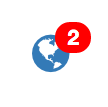
\includegraphics[height=1.5cm]{images/skedge/social-note1}
        \caption{\emph{Pending share requests} notification} \label{fig:sk-social-note1}
      \end{subfigure}

      \hspace{20pt}
      
      \begin{subfigure}[w]{6.5cm}
        \centering
        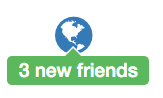
\includegraphics[height=1.5cm]{images/skedge/social-note2}
        \caption{\emph{New friends} notification} \label{fig:sk-social-note2}
      \end{subfigure}
    \end{tabular}
    \caption{Notifications: none, one, or both of them can adorn the Skedge Social logo}
  \end{figure}

